% !TEX root = ../topk_thesis.tex
%% Copyright 1998 Pepe Kubon
%%
%% `one.tex' --- 1st chapter for thes-full.tex, thes-short-tex from
%%                the `csthesis' bundle
%%
%% You are allowed to distribute this file together with all files
%% mentioned in READ.ME.
%%
%% You are not allowed to modify its contents.
%%

%%%%%%%%%%%%%%%%%%%%%%%%%%%%%%%%%%%%%%%%%%%%%%%%%
%
%       Chapter 1 
%
%%%%%%%%%%%%%%%%%%%%%%%%%%%%%%%%%%%%%%%%%%%%%%%%

\chapter{Introduction}

In this chapter, we first introduce the basic idea of skyline subspace problem and several interesting applications that motivate the problem, which will be studied in this thesis. Then, we will summarize the major contributions and describe the structure of the thesis.

\section{Motivations}
The skyline operator is an important research topic for multi-criteria decision making applications.

One classic example of skyline queries is searching for hotels that are cheap and close to the beach~\cite{borzsony2001skyline}. We assume that each hotel has two attributes: the price and the distance from the hotel to the beach.
Suppose there is Hotel A and Hotel B and the price of Hotel A is lower than the price of Hotel B, The distance from Hotel A to the beach is also shorter than the distance from Hotel B to beach.
Then Hotel A dominates Hotel B.
We call those hotels that are not dominated by others in terms of price and distance to the beach skyline hotels. 
There are many recent studies on efficient methods for skyline computation, subspace skyline analysis and skyline computation in different scenarios.

However, all the previous studies are about the skyline computation. The questions about computing the subspaces of query point with respect to skyline remain open.

\begin{figure}[H]
\centering
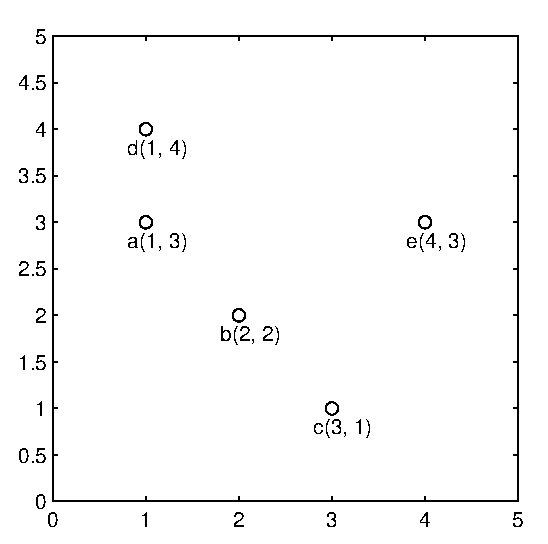
\includegraphics[width=0.5\textwidth]{figs/intro_xy.eps}
\caption{An example of data points on full space $(X, Y)$}
\label{fig:intro_xy}
\end{figure}

\begin{figure}[H]
\centering
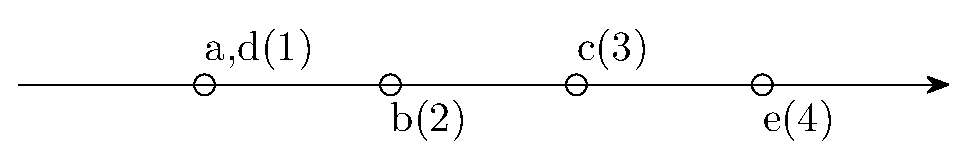
\includegraphics[width=0.5\textwidth]{figs/intro_x.eps}
\caption{The projection of data points on subspace $X$}
\label{fig:intro_x}
\end{figure}

\begin{figure}[H]
\centering
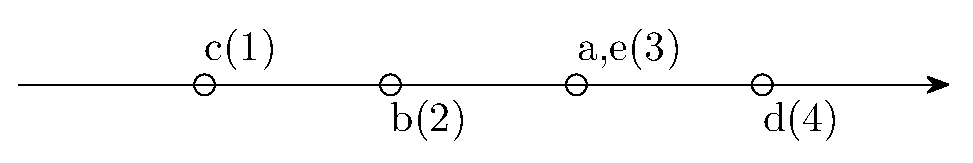
\includegraphics[width=0.5\textwidth]{figs/intro_y.eps}
\caption{The projection of data points on subspace $Y$}
\label{fig:intro_y}
\end{figure}

\begin{example} 
\label{exp:xy:points}
Consider a set of $5$ data points in 2-d space $(X, Y)$ as shown in Figure~\ref{fig:intro_xy}. The points $a$, $b$ and $c$ are skyline points in space $(X, Y)$ since each of them is not dominated by any other points.
\end{example}

In Figure~\ref{fig:intro_x} and Figure~\ref{fig:intro_y}, we also plot the projections of the data points on dimensions $X$ and $Y$, respectively. In our thesis, we are only interested in the non-trivial subspaces that are non-empty. In Example~\ref{exp:xy:points}, subspace $X$ and subspace $Y$ are two non-empty subspaces that we are interested in. In subspace $X$, the projections of the point $a$ and $d$ have the same value. Both of them are subspace skyline points of subspace $X$. In subspace $Y$, the projection of point $c$ is also a skyline point.

From Figure~\ref{fig:intro_xy}, we can see that point $a$, point $b$ and point $c$ are skyline points in the full space $(X, Y)$. However, there are differences among them if we look at them in different projections. Point $a$ is a subspace skyline point in subspace $X$. Point $c$ is a subspace skyline point in subspace $Y$. Although $b$ is also skyline point in the full space $(X, Y)$, it is not skyline point neither in projection $X$ nor in projection $Y$.

Taking the value $1$ on subspace $Y$ is sufficient for $c$ to be a skyline point in the full space $(X, Y)$. No other points are able to dominate $c$ because $c$ is the only point with the minimal value $1$ on subspace $Y$. While taking the value $1$ on subspace $X$ is not sufficient for $a$ to be a skyline point in full space, because $d$ also has the same minimal value $1$ on subspace $X$. Point $b$ does not have minimal value on subspace $X$ or subspace $Y$.

Point $d$ and $e$ are still subtly different although either of them is not a skyline object in full space $(X, Y)$. With the same minimal value $1$ as point $a$ on subspace $X$, point $d$ is a skyline points in subspace $X$. Point $e$ is not a skyline point neither on full space $(X, Y)$ or any subspaces of $(X, Y)$.

In our thesis, we are interested in finding all the minimal subspace projections such that the query point is a skyline point on those projections. We call these projections \emph{skyline subspaces} of the query point.

\emph{Why are we interested about the skyline subspaces of the query points?} The information of skyline subspace helps us understand the data better. In Section~\ref{ch:exp:graph}, we analyze a real data set of DBLP citation network. We take the distances between all authors and all conferences as criteria and compute the subspaces on which the query author point is a skyline point. By computing those subspaces, we are able to know what distinguishes an author from its peers in terms of research topics and academic connections of that author. For example, an author publishes papers or connects with other authors who publish papers in all quantum computing conferences $A$, $B$, $C$ and $D$. If this author is a skyline points in terms of connections and publications in these four conferences, then we say that this author has a good reputations in quantum computing. We are interested in the subsets of these conferences that make this author distinguished with others. In Section~\ref{ch:exp:spatial}, we analyze the Yelp academic dataset. Given a query business spot, taking the Euclidean distances between the business spots and the business categories (restaurant, coffee shop, etc.) as criteria, we are interested in finding the sets of business categories that makes the business spot special.

Computing the skyline points of all the subspaces~\cite{pei2005catching, yuan2005efficient} is costly when user are only interested in finding subspaces of a certain the query points. In this thesis, we are focusing on skyline subspaces of one query point but not the whole dataset also known as \emph{skyline membership queries} in \cite{pei2005catching}.

\section{Contributions}
The original skyline operator problems have been studied in~\cite{borzsony2001skyline, chomicki2003skyline} and subspace skyline problems have been studied in~\cite{pei2005catching, yuan2005efficient}. In this thesis, our goal is to find the subspaces where the query point is in the subspace skylines. By tackling this problem. We make the following contributions.

\begin{itemize}
\item We develop an algorithm framework to answer the \emph{skyline subspace query}, finding the subspaces where the query point is in the subspace skyline. We present a bottom-up algorithm based on set enumeration and dominant candidate sets intersection to solve the problem.

\item We apply skyline subspace query on two specific applications: Computing skyline subspaces on graph and computing the skyline subspaces on Euclidean space. We develop effective pruning algorithms to reduce the unnecessary computation.

\item A performance study using both synthetic and real data sets is conducted to evaluate our approach. For the skyline subspace problem on the graph, we run our algorithm on DBLP citation network to test its efficiency and scalability. For the spatial skyline subspace problem, we run our algorithm on YELP academic dataset.
\end{itemize}
  

\section{Organization of the Thesis}
The rest of the thesis is organized as follows. In Chapter~\ref{ch:related-work}, we review the related work of skyline queries. We then formulate our \emph{skyline subspace} problem in Chapter~\ref{ch:prob-def}. In Chapter~\ref{ch:graph}, we propose the basic framework of our algorithm and the pruning method on \emph{skyline subspace query on graph}.  In Chapter~\ref{ch:spatial}, we present our algorithm of \emph{spatial skyline subspace query}.  We report our experimental results in Chapter~\ref{ch:exp}, and conclude the thesis in Chapter~\ref{ch:con}.










